\chapter{Methodology}
\section{Introduction}
A systematic review is a rigorous and structured research method designed to comprehensively identify, evaluate, and synthesize all available evidence relevant to a clearly formulated research question. Unlike narrative reviews, which may be more descriptive and selective, systematic reviews follow transparent, replicable procedures to minimize bias and ensure reliability \cite{higgins2011cochrane,liberati2009prisma}. This process involves the development of predefined inclusion and exclusion criteria, a systematic search strategy, critical appraisal of eligible studies, and structured data synthesis. This study adopts a systematic review approach, guided by the Preferred Reporting Items for Systematic Reviews and Meta-Analyses (PRISMA) framework, to ensure that findings on workplace stress, dietary choices, and physical activity in relation to metabolic syndrome are comprehensive, unbiased, and evidence-based \cite{moher2009,page2021prisma}.



\section{ Eligibility criteria}
Employing the 'PCC' acronym, Population, Concept, Context, as suggested for qualitative syntheses \cite{lockwood2017}, studies were included in this review if they fulfilled the following criteria:\\
\textbf{Population:} Adults of working age (generally 18-65 years) who are either formally employed or working in workplace settings, with or without a clinical diagnosis of metabolic syndrome. In addition, populations are at risk of developing metabolic syndrome due to occupational and lifestyle determinants. \\
\textbf{Concept:} The impact of occupational stress, diet, and physical activity level on metabolic health. This encompasses how chronic stress, unhealthy diet, and lack of exercise play a role in the development or control of metabolic syndrome and its corresponding features (i.e., central obesity, insulin resistance, dyslipidemia, and hypertension). \\
\textbf{Context:} Work settings and everyday life settings in which occupational stress, diet, and physical activity patterns are set, e.g., office-based work, shift work, working from home, or other work settings. Research from high-income and low- to middle-income countries was included to represent varying lifestyle and work environment conditions. \\
\textbf{Study designs:} The review comprised peer-reviewed studies with qualitative, quantitative, or mixed-method designs that examined the contribution of workplace stress, diet, and physical activity to the development of metabolic syndrome. Excluded were non-research articles, such as editorials, conference abstracts, study protocols, and grey literature, to include rigorously developed and relevant evidence.

\section{ Search strategy}
In February 2025, an extensive search was performed on English-language articles published from 2015 to 2025, using multiple reputable databases including PubMed MEDLINE, Scopus and Science Direct. Various search terms were employed and applied consistently across all databases. These terms included: (Workplace stress or Dietary Choices or Physical Activity) AND (Metabolic Syndrome). The same combinations of search terms were utilized for the other databases. 
\section{ Study Selection Criteria }
This study included original research investigations that met the following criteria: (1) incorporation of elements related to metabolic syndrome; (2) intention to assess the impact of physical activity, dietary choices, and / or workplace stress on metabolic syndrome; (3) Classification as primary studies employing Randomized Controlled Trial. Conversely, studies were excluded if they: (1) were solely available in abstract form without access to the full text; (2) were studies not published in English Language. 

\section{Data extraction and data synthesis }
After the searches were completed, all identified citations were obtained. Then, reference management
software like excel, used with
proper copyright authorization, was utilized to remove any duplicate entries. Subsequently, the titles and
abstracts of each article were extracted from the reference manager and imported into an excel spreadsheet for further analysis.\par
 Before starting the screening process, preliminary screenings were performed. This screening procedure was carried out independently by four evaluators. subsequently, pertinent information meticulously extracted from each study, including the author, publication year, age range, gender, measure tools used, dietary patterns, components assessed and key results.
 
\section{Assessment of trustworthiness}
To ensure the trustworthiness and rigor of this systematic review, several strategies were employed. \par
Initially, only original research studies published in peer-reviewed journals were included. The selection process was guided by clearly defined inclusion and exclusion criteria to ensure that the findings reflect a reliable and accurate understanding of the relationship between workplace stress, dietary habits, physical activity, and metabolic syndrome.\par
Efforts were made to minimize researcher bias by maintaining transparency in the review process. The use of the PRISMA guidelines provided a structured approach to documentation and reporting. Additionally, decisions regarding study inclusion, data extraction, and synthesis were verified by multiple reviewers ensuring that interpretations were grounded in the data. The PRISMA framework is shown in Figure ~ \ref{fig:prisma-flow-diagram1} below.\\


\begin{figure}[H]
    \centering
    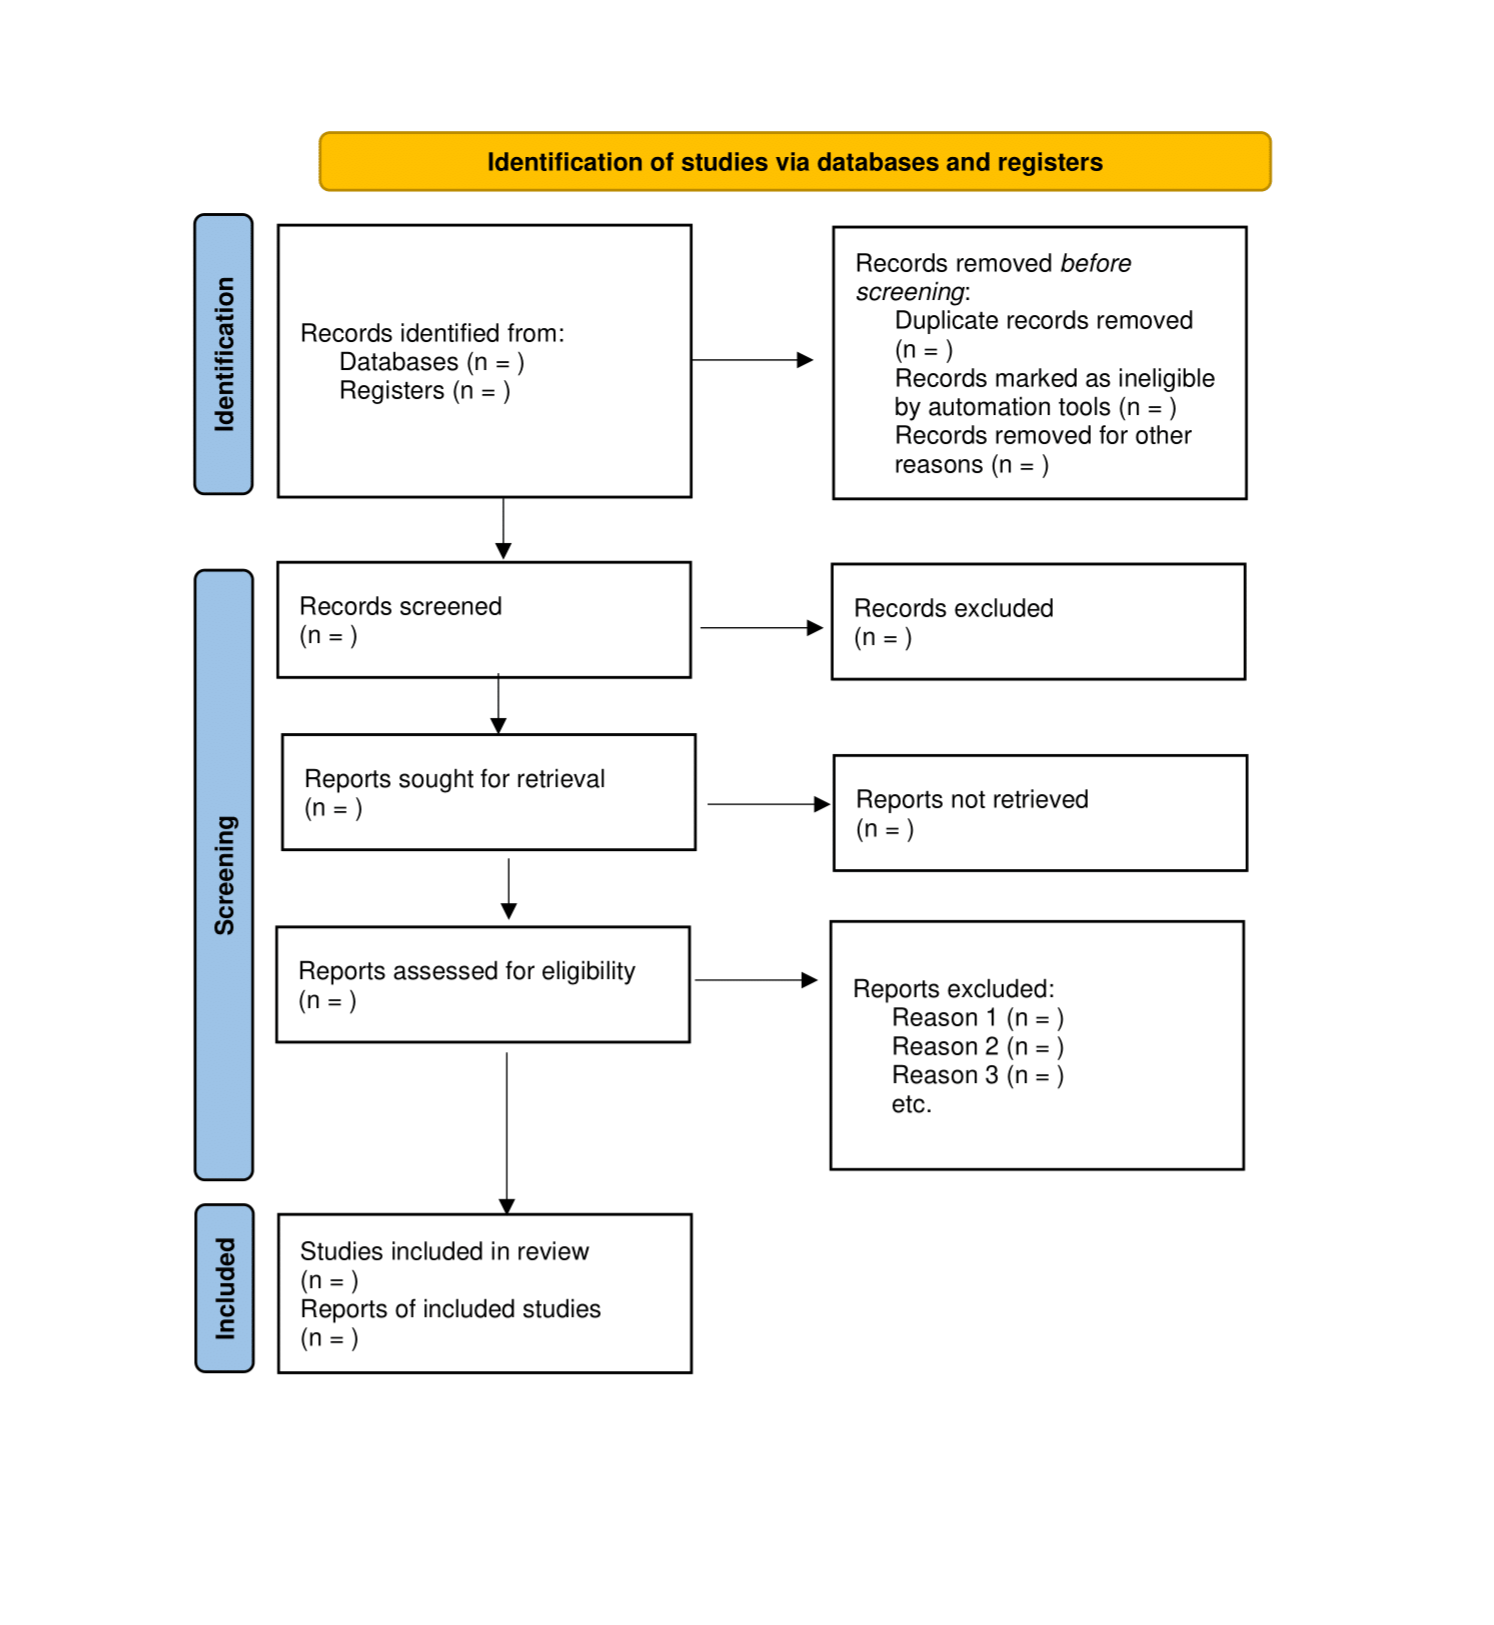
\includegraphics[width=\linewidth]{PRISMA FLOW CHART.PNG}
    \caption{Number of Publications by Year}
    \label{fig:prisma-flow-diagram1}
\end{figure}





